\chapter{Assesment of Transcriptional Induction, Expression, and Subcellular Localisation of Bovine IFITs in the Context of RSV} \label{Assesment of Transcriptional Induction, Expression, and Subcellular Localisation of Bovine IFITs in the Context of RSV}
\section{Introduction and Aims} \label{Introduction and Aims}
\textbf{Half page intro:}
about cross species interaction + question about lab attenuated or not the brsv stuff
\textbf{Half page aims:}
We hypothesised both human and bovine IFITs to be induced by human and bovine RSV infection. We aimed to systematically test this by initially confirming that our model cell lines are capable of IFIT induction following the treatment of known innate immune system activators such as interferons, LPS, and poly I:C. We would then assess the IFIT induction during human and bovine RSV infection using a range of viral concentration and end assay time points. Lastly, we would validate this data in more physiologically relevant cell lines as well as using omics approaches.

\section{Results} \label{Results}
\subsection{Technologies} \label{Technologies}
\subsubsection{Bovine \textit{IFIT} qPCR Primer Validation} \label{Bovine IFIT qPCR Primer Validation}
Due to the initial lack of commercially available primers for the detection of bovine \textit{IFIT} transcripts at the outset of the project, I devised a panel comprising three primer sets (PS) for each bovine \textit{IFIT} gene. Detailed information about this process is outlined in Section \ref{Primer Design and Assay Setup}. In a nutshell, I inputted the coding sequences into the PrimerQuest software (Integrated DNA Technologies) to identify the most suitable oligonucleotides. To evaluate the amplification efficiencies of each primer set, I employed \textit{IFIT} DNA clones from a bovine ISG library as standards (accessible through a collaboration with CVR Glasgow). The outcomes are depicted in Figure \ref{Validation of custom-made bIFIT qPCR primers}. The graph demonstrates that primer sets 1 exhibited the most favourable amplification efficiencies. All primer sets, except for \textit{bIFIT3}, yielded nearly impeccable amplification efficiencies of around 100\%. Consequently, they were chosen for subsequent experiments. While \textit{bIFIT3} primer sets demonstrated similar outcomes in terms of standard curve slopes and amplification efficiencies, PS1 consistently outperformed the others in repeated testing rounds (data not presented). As a result, it was singled out for further experimentation.

\begin{figure}
    \centering
    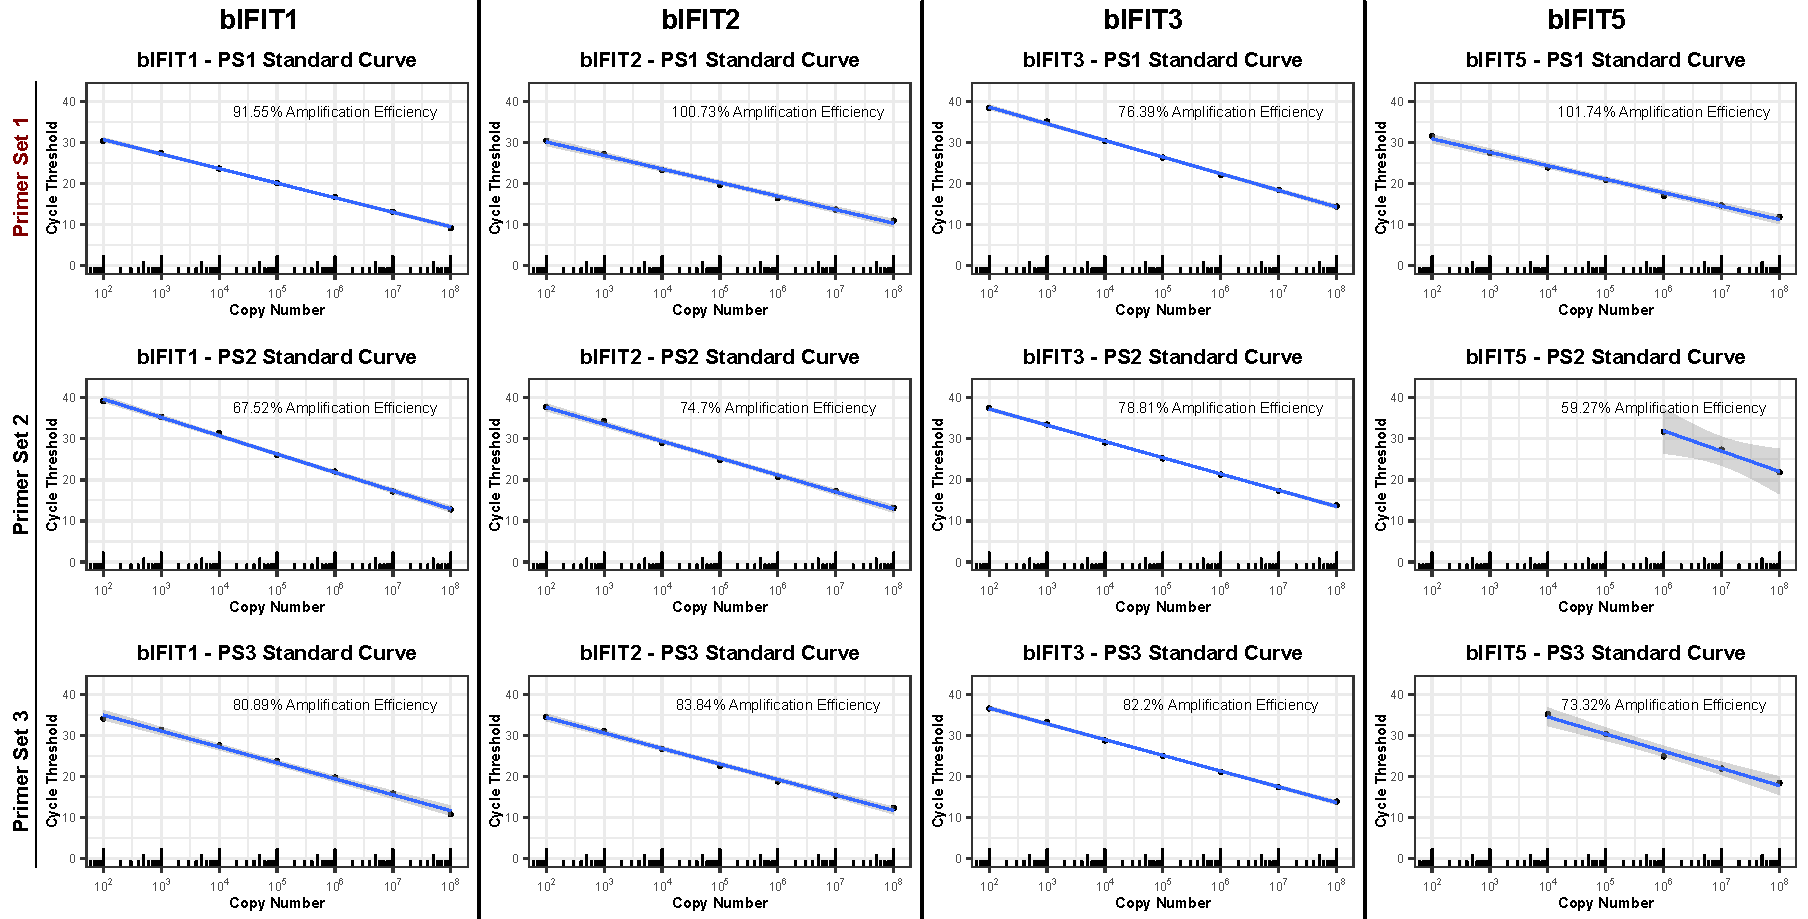
\includegraphics[width=1\linewidth]{07. Chapter 2/Figs/01. Technologies/02. primer validation.pdf}
    \caption[Validation of Custom-Made \textit{bIFIT} qPCR Primers.]{\textbf{Validation of Custom-Made \textit{bIFIT} qPCR Primers.} The custom-designed primers were evaluated by creating a serial dilution of bovine \textit{IFIT}-containing plasmids, provided by the CVR Glasgow. The resulting standard curves are shown here. Primer set (PS) 1 (a), 2 (b), and 3 (c) are depicted for bovine \textit{IFIT1} (1.), \textit{IFIT2} (2.), \textit{IFIT3} (3.), and \textit{IFIT5} (4.), along with their calculated amplification efficiencies.}
    \label{Validation of custom-made bIFIT qPCR primers}
\end{figure}

The PSs behaviour was monitored throughout the project, as fresh standard curves were created per experiment. Figure \ref{The Performance of Custom-Made Primer-Sets Over Time} shows that the average data is consistent with what was observed in initial testing (Figure \ref{Validation of custom-made bIFIT qPCR primers}), however, there were per experiment deviations in slope angles for each of the selected primer pairs. The underlying amplification efficiencies stayed consistent, as is highlighted by the averaged efficiencies displayed. The initial \textit{bIFIT3} PSs differential amplification slopes compared to the other \textit{bIFIT} PSs, as well as the variable nature of PSs performance throughout the project prohibits the usage of \(\Delta\)\(\Delta\)Ct methodologies for transcript quantification as the increase in cycle threshold would not be proportional to the decrease of transcript abundance between the \textit{bIFITs}, and thus a different methodology had to be adopted. This is described in detail in Section \ref{Data Processing}. In short, the copy numbers were deducted from standard curves and factorised by the relative abundance of bovine \textit{GAPDH}. This ensured the slope-independent establishment of relative expression values, mirroring and complementing data from \(\Delta\)\(\Delta\)Ct methodologies.

\begin{figure}
    \centering
    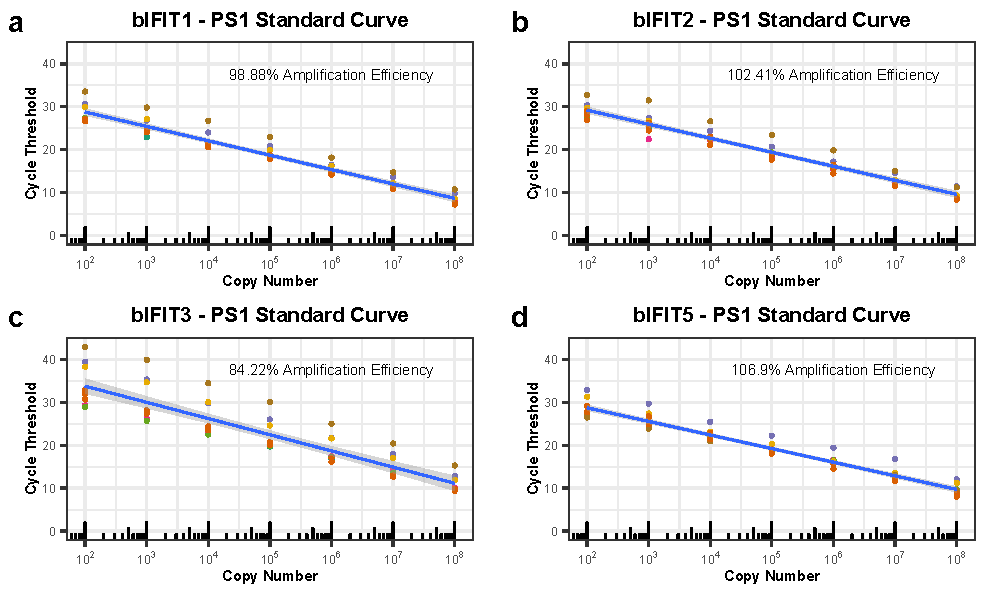
\includegraphics[width=1\linewidth]{07. Chapter 2/Figs/01. Technologies/03. standard curves behaviour.pdf}
    \caption[The Performance of Custom-Made Primer-Sets Over Time.]{\textbf{The Performance of Custom-Made Primer-Sets Over Time.} During the experiments with custom-made \textit{bIFIT} qPCR primers, standard curves had to be always constructed. Here, the underlying average amplification efficiencies and standard curves, along with the individual data, from all the experiments and coloured by the experiment are displayed.}
    \label{The Performance of Custom-Made Primer-Sets Over Time}
\end{figure}

\subsubsection{Growth curves of bovine RSV in bovine cell lines} \label{Growth curves of bovine RSV in bovine cell lines}
Describe data: \newline
asdasdasd \newline
This was done as a complement to existing data done by other people in Dalan’s group on human cell lines with hRSV growth curves. The novelty is especially growth curves in BT cells. I do not know if I totally knew what I was doing at the time, so I do not know how much to trust this data.  

\begin{figure}
    \centering
    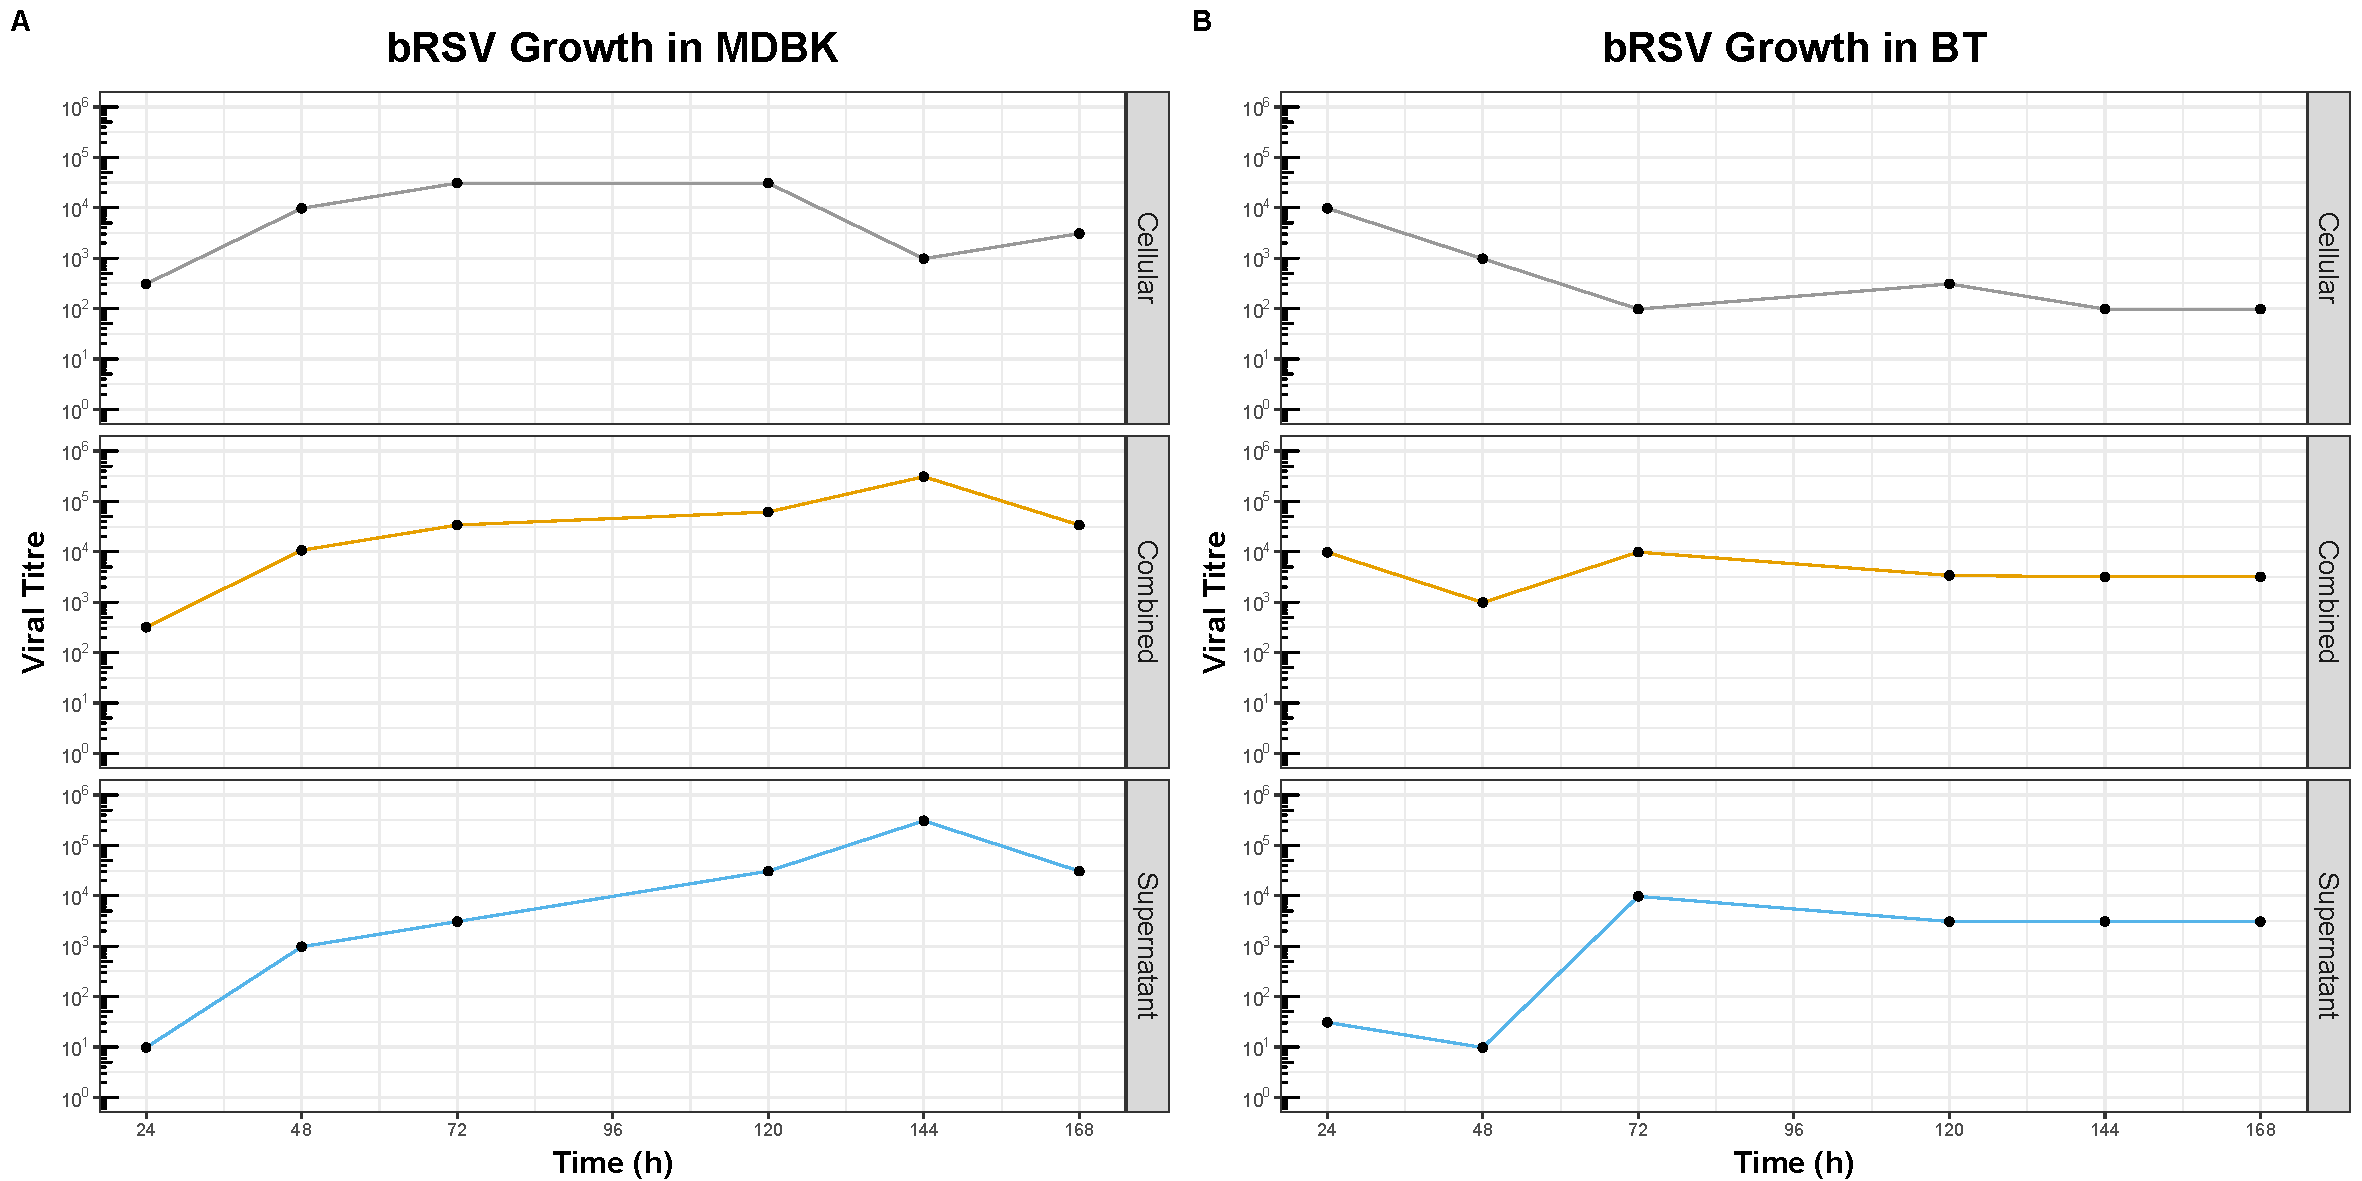
\includegraphics[width=1\linewidth]{07. Chapter 2/Figs/01. Technologies/01. growth_curves.pdf}
    \caption[bRSV growth curves in MDBK and BT cell lines.]{\textbf{bRSV growth curves in MDBK and BT cell lines.} sdfgsdfg sdfg sdfg sdfg sdfg sdfg }
    \label{bRSV growth curves in MDBK and BT cell lines}
\end{figure}


\section{Discussion} \label{Discussion}
Recap human \newline
Recap bovine \newline
Bovine rna seq studies